\documentclass[11pt]{article}
\usepackage{graphicx}
\usepackage{float}
\usepackage{listings}
\usepackage{caption}
\usepackage{amsmath}
\usepackage{listings}
\usepackage{xcolor}
\usepackage[top = 0.7in,bottom = 1in, left = 0.8in, right = 0.8in]{geometry} 

%New colors defined below
\definecolor{codegreen}{rgb}{0,0.6,0}
\definecolor{codegray}{rgb}{0.5,0.5,0.5}
\definecolor{codepurple}{rgb}{0.58,0,0.82}
\definecolor{backcolour}{rgb}{0.95,0.95,0.92}

%Code listing style named "mystyle"
\lstdefinestyle{mystyle}{
  backgroundcolor=\color{backcolour},   commentstyle=\color{codegreen},
  keywordstyle=\color{magenta},
  numberstyle=\tiny\color{codegray},
  stringstyle=\color{codepurple},
  basicstyle=\ttfamily\footnotesize,
  breakatwhitespace=false,         
  breaklines=true,                 
  captionpos=b,                    
  keepspaces=true,                 
  numbers=left,                    
  numbersep=5pt,                  
  showspaces=false,                
  showstringspaces=false,
  showtabs=false,                  
  tabsize=2
} 
\lstset{style=mystyle}

\title{\textbf{CS747 : Programming Assignment 2}}
\author{\textbf{Adityaya Dhande}   \hspace{8mm} \textbf{210070005}}
\begin{document}
\maketitle
\section*{Task 1}

\subsection*{UCB}

\begin{figure}[H]
    \begin{center}
        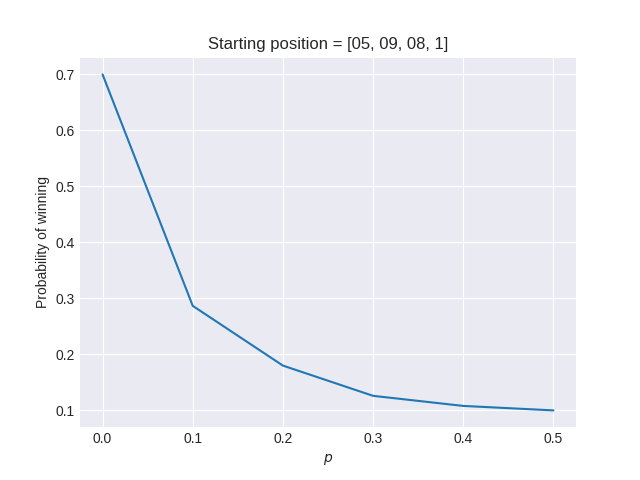
\includegraphics[width=0.8\textwidth]{../images/plot1.png}
        
        \caption{Regret vs Horizon for UCB algorithm}
    \end{center}
 \end{figure}
 Regret increases with horizon as expected and follows a logarithmic variation
 \begin{lstlisting}[language=Python]      
    class UCB(Algorithm):
    def __init__(self, num_arms, horizon):
        super().__init__(num_arms, horizon)
        self.ucbs = np.zeros(num_arms)
        self.u = np.zeros(num_arms)
        self.p_hat = np.zeros(num_arms)
    
    def give_pull(self):
        t = sum(self.u)
        self.ucbs = self.p_hat + np.sqrt(2 * np.log(t) / self.u)
        return np.argmax(self.ucbs)
    
    def get_reward(self, arm_index, reward):
        self.u[arm_index] += 1
        n = self.u[arm_index]
        mean = self.p_hat[arm_index]
        new_mean = ((n - 1) / n) * mean + (reward / n)
        self.p_hat[arm_index] = new_mean\end{lstlisting}
    \textbf{Code explanation :} \texttt{self.ucbs} is an array containing
    the UCBs of all the arms in a given iteration. \texttt{self.u} contains
    the number of times each arm has been pulled till the current iteration. 
    \texttt{self.p\_hat} contains the empirical means of all the arms
    based on pulls till the current iteration. 
    
    \noindent The \texttt{get\_reward} function
    takes the index of the arm which was pulled and the reward and increments 
    \texttt{self.u[arm\_index]} by 1 because that arm was pulled in this iteration, 
    and thus the total number of pulls of that arm has increased by 1. 
    If now the total number of pulls is $n$ then the old number of pulls was
    $n-1$, and thus the total reward before the current pull was 
    $\text{old mean}\times(n-1)$. The new mean is 
    $$\text{new mean} = \frac{\text{total reward}}{\text{total number of pulls}} = \frac{\text{total reward before current pull + reward of current pull}}{\text{total number of pulls}}$$
    The new mean is set for the arm that was pulled.

   \noindent The \texttt{give\_pull} function calculates the UCB 
   for each arm as $ucb_a^t = \hat{p}_a^t + \sqrt{\frac{2 \ln(t)}{u_a^t}}$
    and returns the index of the arm with the maximum UCB.

    \vspace{3mm}
   \subsection*{KL-UCB}
 \begin{figure}[H]
    \begin{center}
        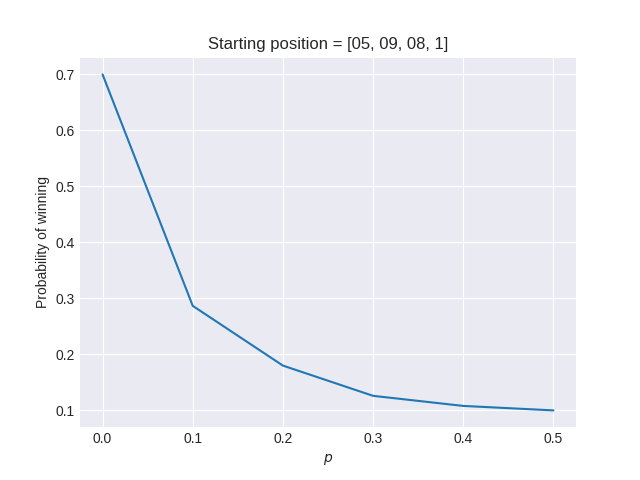
\includegraphics[width=0.8\textwidth]{../images/plot1.png}
        
        \caption{Regret vs Horizon for KL-UCB}
    \end{center}
 \end{figure} 
 Regret increases with horizon as expected and follows a logarithmic variation. The decrease
 in the end can be explained by negative regret generated because of the optimal arm being pulled many times.
 \begin{lstlisting}[language=Python]      
    def KL(x ,y):
    if x == 0 :
        return math.log(1/(1 - y))
    elif x == 1 :
        return math.log(1/y)
    return (x * math.log(x / y) + (1 - x) * math.log((1 - x) / (1 - y)))

    def KL_ucb(p, u_a, t, c = 3, tol = 1e-3) : 
        l = p
        u = 1
        q = (l + u)/2   
        target = (math.log(t) + c * math.log(math.log(t)))/u_a
        while (u - l > tol):
            q = (l + u)/2
            current = KL(p,q)
            if current < target :
                l = q
            elif current > target :
                u = q
            else :
                return q
        return q  

    class KL_UCB(Algorithm):
    def __init__(self, num_arms, horizon):
        super().__init__(num_arms, horizon)
        self.first_pull = True
        self.kl_ucbs = np.zeros(num_arms)
        self.u = np.zeros(num_arms)
        self.p_hat = np.zeros(num_arms)
    
    def give_pull(self):
        if self.first_pull :
            arm = int(sum(self.u))
            if arm == (len(self.kl_ucbs) - 1) :
                self.first_pull = False
            return arm
        t = sum(self.u)
        for i in range(len(self.kl_ucbs)):
            self.kl_ucbs[i] = KL_ucb(self.p_hat[i], self.u[i], t, c=0)
        arm = np.argmax(self.kl_ucbs)
        return arm
    
    def get_reward(self, arm_index, reward):
        self.u[arm_index] += 1
        n = self.u[arm_index]
        mean = self.p_hat[arm_index]
        new_mean = ((n - 1) / n) * mean + (reward / n)
        self.p_hat[arm_index] = new_mean\end{lstlisting}
    \noindent
    \textbf{Code explanation :}\texttt{self.first\_pull} is a boolean variable
    which is \texttt{True} till all the arms have been sampled for the first time.
     \texttt{self.kl\_ucbs} is an array containing
    the KL-UCBs of all the arms in a given iteration. \texttt{self.u} contains
    the number of times each arm has been pulled till the current iteration. 
    \texttt{self.p\_hat} contains the empirical means of all the arms
    based on pulls till the current iteration. 

    
    \noindent The \texttt{get\_reward} function
    takes the index of the arm which was pulled and the reward and increments 
    \texttt{self.u[arm\_index]} by 1 because that arm was pulled in this iteration, 
    and thus the total number of pulls of that arm has increased by 1. 
    If now the total number of pulls is $n$ then the old number of pulls was
    $n-1$, and thus the total reward before the current pull was 
    $\text{old mean}\times(n-1)$. The new mean is 
    $$\text{new mean} = \frac{\text{total reward}}{\text{total number of pulls}} = \frac{\text{total reward before current pull + reward of current pull}}{\text{total number of pulls}}$$
    The new mean is set for the arm that was pulled.

   \noindent The \texttt{give\_pull} function samples each arm once for the first \texttt{num\_arms} times. 
    From then on it calculates the KL-UCB for each arm as $q$ \text{such that }
    $$\texttt{self.u[arm\_index]}\times KL(\texttt{self.p\_hat[arm\_index]}, q) = \ln(t) + c \ln(\ln(t))$$ and returns 
    the index of the arm with the highest KL-UCB. The value of $c$ used here is 0. The value of $q$ is
    found using binary search because $KL(p,p) = 0$ and $KL(p,1) = \infty$ and it increases as the second argument increases
    from $p$ to 1. The function \texttt{KL\_ucb} does exactly this with a tolerance in the value of q 
    of about $10^{-3}$. The function \texttt{KL(x,y)} returns the KL divergence of 2 bernoulli distributions 
    with means \texttt{x} and \texttt{y}.

\subsection*{Thompson Sampling}
 \begin{figure}[H]
    \begin{center}
        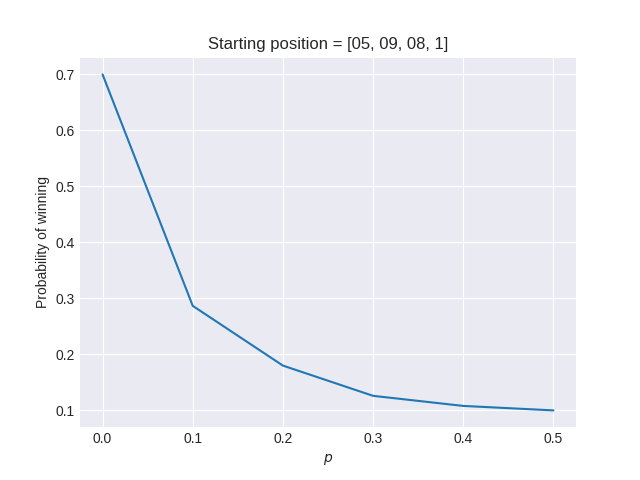
\includegraphics[width=0.8\textwidth]{../images/plot1.png}
        \caption{Regret vs Horizon for Thompson Sampling}
    \end{center}
 \end{figure}
 Regret increases with horizon as expected 

 \begin{lstlisting}[language=Python]      
    class Thompson_Sampling(Algorithm):
    def __init__(self, num_arms, horizon):
        super().__init__(num_arms, horizon)
        self.sa = np.zeros(num_arms)
        self.fa = np.zeros(num_arms)
        self.t_samples = np.zeros(num_arms)
    
    def give_pull(self):
        for i in range(len(self.t_samples)) :
            self.t_samples[i] = np.random.beta(self.sa[i] + 1, self.fa[i] + 1)
        return np.argmax(self.t_samples)
    
    def get_reward(self, arm_index, reward):
        self.sa[arm_index] += reward
        self.fa[arm_index] += 1 - reward        \end{lstlisting}
    
\noindent
\textbf{Code explanation :} \texttt{self.sa} stores the number of successes(reward=1) of 
all the arms until the current iteration. \texttt{self.fa} stores the number of failures(reward=0) of 
all the arms until the current iteration. \texttt{self.t\_samples} stores 
the samples drawn from the beta distribution corresponding to each arm. 

\noindent The \texttt{get\_reward} function takes the arm index and the reward and increases the successes of
that arm by 1 if the reward is 1 and increases the failures of that arm by 1 if the reward is 0

\noindent The \texttt{give\_pull} function draws, for each arm, samples from 
$$\beta(\texttt{self.sa[arm\_index]}+1,\texttt{self.fa\_[arm\_idex]}+1)$$
and returns the index of the arm whose $\beta$ distribution gives the greatest sample.

\end{document}
 